\section{Methodologies}

\subsection{Model definition}

\begin{frame}[allowframebreaks]{Universal differential equation}
    \gls{UDE} \cite{rackauckasUniversalDifferentialEquations2020} is based on \gls{NeuralODE}

    \begin{block}{Generalized \gls{UDE}}
        \begin{equation*}
            u' = f(u, t, U_\theta(u, t))
        \end{equation*}
    \end{block}

    \framebreak

    \begin{block}{UDE system}
        \begin{equation*}
            \begin{aligned}
                S' &= - \frac{\beta(t) SI}{N} \\
                E' &= \frac{\beta(t) SI}{N} - \gamma E \\
                I' &= \gamma E - \lambda I \\
                R' &= (1 - \alpha(t)) * \lambda * I \\
                D' &= \alpha(t) * \lambda * I \\
                N' &= - \alpha * \lambda * I \\
                C' &= -C + \gamma * E \\
                T' &= \gamma * E \\
            \end{aligned}
        \end{equation*}
    \end{block}

    \framebreak

    \begin{block}{UDE system}
        \begin{equation*}
            \begin{aligned}
                \beta(t) &= \mathcal{NN}_{\theta_1}(\mathcal{F}) \\
                \alpha(t) &= \mathcal{NN}_{\theta_2} (\frac{t}{t_\text{max}}, \frac{I(t-1)}{N(t-1)}, \frac{R(t-1)}{N(t-1)}, \frac{D(t-1)}{N(t-1)})
            \end{aligned}
        \end{equation*}
    \end{block}

    \begin{itemize}
        \item Hidden layers activation: mish \cite{misraMishSelfRegularized2020}
        \item Output layer activation $\nu_i = \nu_{i,L} + (\nu_{i,U} - \nu_{i,L}) * \sigma (z_i)$
    \end{itemize}

    \framebreak

    \begin{block}{Set of covariates 01}
        \begin{equation*}
            \begin{aligned}
                \mathcal{F}_1(t) = \left\lbrace \frac{t}{t_\text{max}}, \frac{S(t-1)}{N(t-1)}, \frac{E(t-1)}{N(t-1)}, \frac{I(t-1)}{N(t-1)} \right\rbrace,
            \end{aligned}
        \end{equation*}
    \end{block}

    \begin{block}{Set of covariates 02}
        \begin{equation*}
            \mathcal{F}_2(t) = \mathcal{F}_1(t) \cup \left\lbrace \text{MovementRange}(t) \right\rbrace,
        \end{equation*}
    \end{block}

    \begin{block}{Set of covariates 03}
        \begin{equation*}
            \mathcal{F}_3(t) = \mathcal{F}_2(t) \cup \left\lbrace \text{SocialProximityToCases}(t) \right\rbrace,
        \end{equation*}
    \end{block}

\end{frame}

\subsection{Parameters estimation}

\begin{frame}{Loss function}
    Trainable parameters: $(\gamma', \lambda', \theta_1, \theta_2)$
    \begin{block}{Box constraints for system parameters}
        \begin{equation*}
            \begin{aligned}
                \gamma &= \gamma_L + (\gamma_U - \gamma_L) * \sigma (\gamma'), \\
                \lambda &= \lambda_L + (\lambda_U - \lambda_L) * \sigma (\lambda').
            \end{aligned}
        \end{equation*}
    \end{block}

    \begin{block}{Regularized MSE with scaled outputs}
        \begin{equation*}
            \begin{aligned}
            \mathcal{L}(\hat{y}, y)
            &= \frac{1}{T} \sum_{i=1}^N \sum_{t=0}^{T-1} \left[ e^{\zeta t} \left(\frac{\hat{y}_{i,t} - y_{i,t}}{max(y_i) - min(y_i)}\right)^2\right]\\
            &+ \frac{\lambda}{2T} (\Vert\theta_1\Vert^2_2 + \Vert\theta_2\Vert^2_2)
            \end{aligned}
            \label{eq:ude-model-loss}
        \end{equation*}
    \end{block}
\end{frame}

\begin{frame}[allowframebreaks]{Training process}
    \begin{itemize}
        \item Partially observed data for $\lbrace D, C, T \rbrace$
        \item \textit{Tsit5} solver (Tsitouras 5/4 Runge-Kutta method \cite{tsitourasRungeKuttaPairs2011})
        \item \textit{InterpolatingAdjoint} sensitivity algorithm for automatic differentiation
    \end{itemize}

    \framebreak

    \begin{figure}[h]
        \centering
        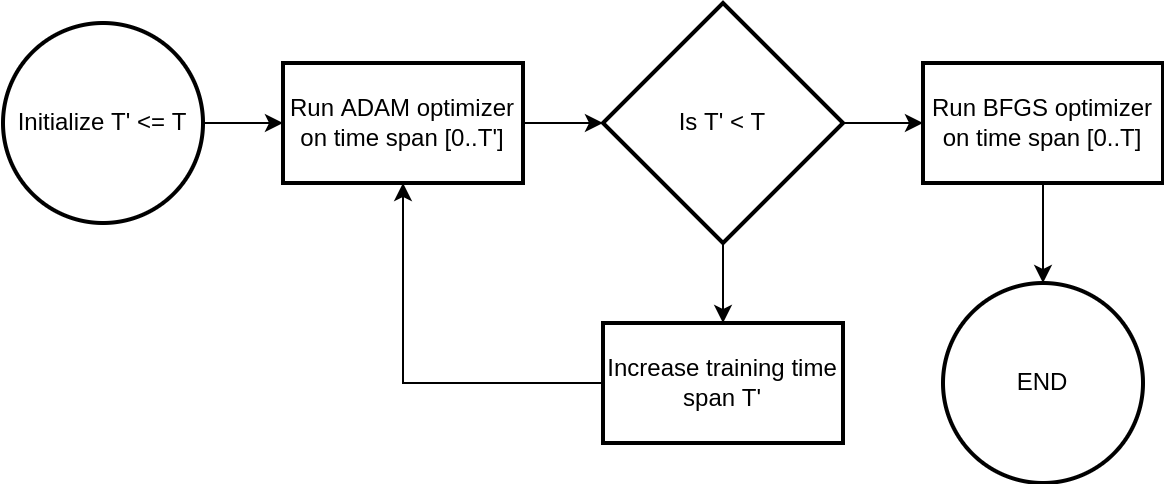
\includegraphics[scale=0.25]{ude-covid19vn-training-flow.png}
        \caption[Training procedure]{Model training procedure}
        \label{fig:model-training-flow}
    \end{figure}

\end{frame}

\subsection{Datasets}

\begin{frame}{Covid-19 cases time series}
    \begin{table}[h]
    \centering
    \begin{tabular}{| c | c | c | c | c |}
        date & infective & confirmed & recoveries & deaths \\
        \hline\hline
        1/22/20 & 0 & 0 & 0 & 0 \\
        \hline
        1/23/20 & 2 & 2 & 0 & 0 \\
        \hline
        1/24/20 & 2 & 2 & 0 & 0 \\
        \hline
        $\cdots$ & $\cdots$ & $\cdots$ & $\cdots$ & $\cdots$ \\
    \end{tabular}
    \caption{Structure of the processed Covid-19 time series datasets}.
    \label{tab:country-covid-timeseries}
    \end{table}

    \begin{itemize}
        \item \gls{JHU} Covid-19 public datasets
        \item \textit{VNExpress} Covid-19 public dashboard
        \item \textit{VnCDC} Covid-19 public dashboard
    \end{itemize}
\end{frame}

\begin{frame}[allowframebreaks]{Facebook's mobility data}

    \begin{table}[h]
    \centering
    \begin{tabular}{| c | c | c | c | c |}
        ds & country & polygon & rel. change & stay put ratio \\
        \hline\hline
        $\cdots$ & $\cdots$ & $\cdots$ & $\cdots$ & $\cdots$ \\
        \hline
        2021-01-01 & VNM & VNM.1.10\_1 & 0.125 & 0.270 \\
        \hline
        2021-01-02 & VNM & VNM.1.10\_1 & 0.052 & 0.259 \\
        \hline
        2021-01-03 & VNM & VNM.1.10\_1 & 0.185 & 0.269 \\
        \hline
        $\cdots$ & $\cdots$ & $\cdots$ & $\cdots$ & $\cdots$ \\
    \end{tabular}
    \caption{Structure of Facebook's Movement Range Maps dataset.}
    \label{tab:facebook-movement-range-maps}
    \end{table}

    \framebreak

    \begin{block}{Social connectedness index}
        \begin{equation*}
            \text{SCI}_{i,j} = \frac{\text{FB connections}_{i,j}}{\text{FB users}_i * \text{FB users}_j},
        \end{equation*}
    \end{block}

    \begin{block}{Social proximity to cases \cite{kuchlerGeographicSpreadCOVID192020}}
        \begin{equation*}
            \text{SPC}_{i,t} = \sum_j^C \text{Cases per 10k}_{j,t} \frac{\text{SCI}_{i,j}}{\sum_h^C \text{SCI}_{i,h}},
        \end{equation*}
    \end{block}

\end{frame}

\begin{frame}{Population data}

    \begin{itemize}
        \item Vietnam: \gls{GSO}
        \item United States: \gls{JHU} Covid-19 datasets
    \end{itemize}

    \begin{table}[h]
    \centering
    \begin{tabular}{| c | c | c |}
        ID\_1 & NAME\_1 & AVGPOPULATION \\
        \hline\hline
        3 & Ha Noi & 8.2466e6 \\
        \hline
        62 & Vinh Phuc & 1.1712e6 \\
        \hline
        16 & Bac Ninh & 1.4191e6 \\
        \hline
        $\cdots$ & $\cdots$ & $\cdots$ \\
        \hline
        1001.0 & Autauga, Alabama, US & 55869 \\
        \hline
        1003.0 & Baldwin, Alabama, US & 223234 \\
        \hline
        1005.0 & Barbour, Alabama, US & 24686 \\
        \hline
        $\cdots$ & $\cdots$ & $\cdots$ \\
    \end{tabular}
    \caption{Structure of the processed average population datasets}.
    \label{tab:country-subdivision-population}
    \end{table}

\end{frame}

\subsection{Experiments}

\begin{frame}[allowframebreaks]{Settings}
    \begin{itemize}
        \item Training period: 48 days
        \begin{itemize}
            \item Vietnam: First date when the total confirmed cases passed 500
            \item United States: 1st July 2021
        \end{itemize}
        \item Testing period: 28 days
        \item ADAM optimizer
        \begin{itemize}
            \item Learning rate 0.05
            \item Weight decay rate 0.5 for each 1000 iterations until 0.00001
            \item 1000 iterations on each time span
            \item Initial time span of 4 days and increased by 4 after each session
        \end{itemize}
        \item BFGS optimizer
        \begin{itemize}
            \item \textit{Initial stepnorm}: 0.01
            \item 1000 iterations on the full time span
        \end{itemize}
    \end{itemize}

    \framebreak

    \begin{itemize}
        \item Apply 7-day moving average to all datasets
        \item Apply min-max scaling on the \glspl{MRM} dataset and \gls{SPC} index
    \end{itemize}

\end{frame}

\begin{frame}[allowframebreaks]{Initial conditions and parameters}

    \begin{table}[h]
        \centering
        \begin{tabular}{| c | c | c | c | c |}
            Location & $S(0)$ & $E(0)$ & $I(0)$ & $R(0)$ \\
            \hline\hline
            Vietnam & 9.75e7 & 25 & 5 & 2817 \\
            \hline
            Ho Chi Minh city & 9.22e6 & 173.5 & 34.7 & 360.1 \\
            \hline
            Binh Duong & 2.58e6 & 206.4 & 41.2 & 314.7 \\
            \hline
            Dong Nai & 3.17e6 & 295 & 59 & 194.8 \\
            \hline
            Long An & 1.71e6 & 217.8 & 43.5 & 300.5 \\
            \hline
            United States & 2.99e8 & 71890 & 14378 & 3.31e7 \\
            \hline
            Los Angeles, California & 8.78e6 & 2500 & 500 & 1.22e6 \\
            \hline
            Cook, Illinois & 4.59e6 & 615 & 123 & 546508 \\
            \hline
            Harris, Texas & 4.30e6 & 930 & 186 & 396430 \\
            \hline
            Maricopa, Arizona & 3.92e6 & 1325 & 265 & 549899 \\
            \hline
        \end{tabular}
        \caption{Initial conditions for the system of ODEs}
        \label{tab:ude-model-initial-conditions}
    \end{table}

    \framebreak

    \begin{table}[h]
        \centering
        \begin{tabular}{| c | c | c | c |}
            Parameter & Value & Lower bound & Upper bound \\
            \hline\hline
            $\beta$ & \textit{N/A} & $0.05$ & $1.67$ \\
            \hline
            $\gamma$ & $1/4$ & $1/4$ & $1/4$ \\
            \hline
            $\lambda$ & $1/14$ & $1/14$ & $1/14$ \\
            \hline
            $\alpha$ & \textit{N/A} & $0.005$ & $0.05$ \\
            \hline
            $\theta_1$ & \textit{glorot\_normal} & \textit{N/A} & \textit{N/A} \\
            \hline
            $\theta_2$ & \textit{glorot\_normal} & \textit{N/A} & \textit{N/A} \\
            \hline
        \end{tabular}
        \caption{Initial parameters for the system of ODEs}
        \label{tab:ude-model-initial-parameters}
    \end{table}

\end{frame}

\subsection{Evaluation metrics}

\begin{frame}{Error functions}

    \begin{block}{Mean absolute error}
        \begin{equation*}
            MAE = \frac{1}{n} \sum_{i=1}^n \left| \hat{y}_i - y_i \right|
        \end{equation*}
    \end{block}

    \begin{block}{Mean absolute percentage error}
        \begin{equation*}
            MAPE = \frac{100}{n} \sum_{i=1}^n \left| \frac{\hat{y}_i - y_i}{y_i} \right|
        \end{equation*}
    \end{block}

    \begin{block}{Root mean squared error}
        \begin{equation*}
            RMSE = \sqrt{\frac{1}{n} \sum_{i=1}{n} (\hat{y}_i - y_i)^2}
        \end{equation*}
    \end{block}

\end{frame}

\subsection{Software and hardware}

\begin{frame}{Software and hardware}

    Julia programming language
    \begin{itemize}
        \item \textit{DifferentialEquations} package
        \item \textit{DiffEqFlux} package
    \end{itemize}

    Linux systems
    \begin{itemize}
        \item Google Cloud Compute \textit{n2-standard-8} instance
        \item Personal laptop with 2-core \textit{Intel(R) Core(TM) i5-4260U} CPU 1.40GHz, and 4Gb of memory.
    \end{itemize}
\end{frame}

\begin{frame}[fragile]{Julia example}
\begin{figure}[!htb]
\centering
\begin{jllisting}
function SEIRD!(du, u, p, t)
    @inbounds begin
        S, E, I, _, _, N, C, _ = u
        β, γ, λ, α = p
        du[1] = -β * S * I / N
        du[2] = β * S * I / N - γ * E
        du[3] = γ * E - λ * I
        du[4] = (1 - α) * λ * I
        du[5] = α * λ * I
        du[6] = -α * λ * I
        du[7] = -C + γ * E
        du[8] = γ * E
    end
    return nothing
end
\end{jllisting}
\caption{Implementation of the system of ODEs in Julia}
\label{fig:diffeq-seird-inplace}
\end{figure}
\end{frame}
